It has been over half a century since renowned astrophysicist Sjur
Refsdal first hypothesized the use of a supernova (SN) resolved into
multiple images as a cosmological tool. In recent years, the first
multiply-imaged core-collapse (CC) SN Refsdal \citep{Kelly:2015a}, and
subsequently the first Type Ia SN iPTF16geu \citep{Goobar:2016}, have
been discovered (Figure 1A-C). As the light for each of the multiple
images follows a different path through the expanding universe and
through the lensing potential, the SN images appear delayed by hours
(for galaxy-scale lenses) or years (for cluster-scale lenses). The
next decade is expected to yield observations of tens to hundreds of
multiply-imaged SNe \citep{Oguri:2010}, yet there is no public
software package for analyzing multiply-imaged SNe.
\begin{wrapfigure}{r}{.5\textwidth}
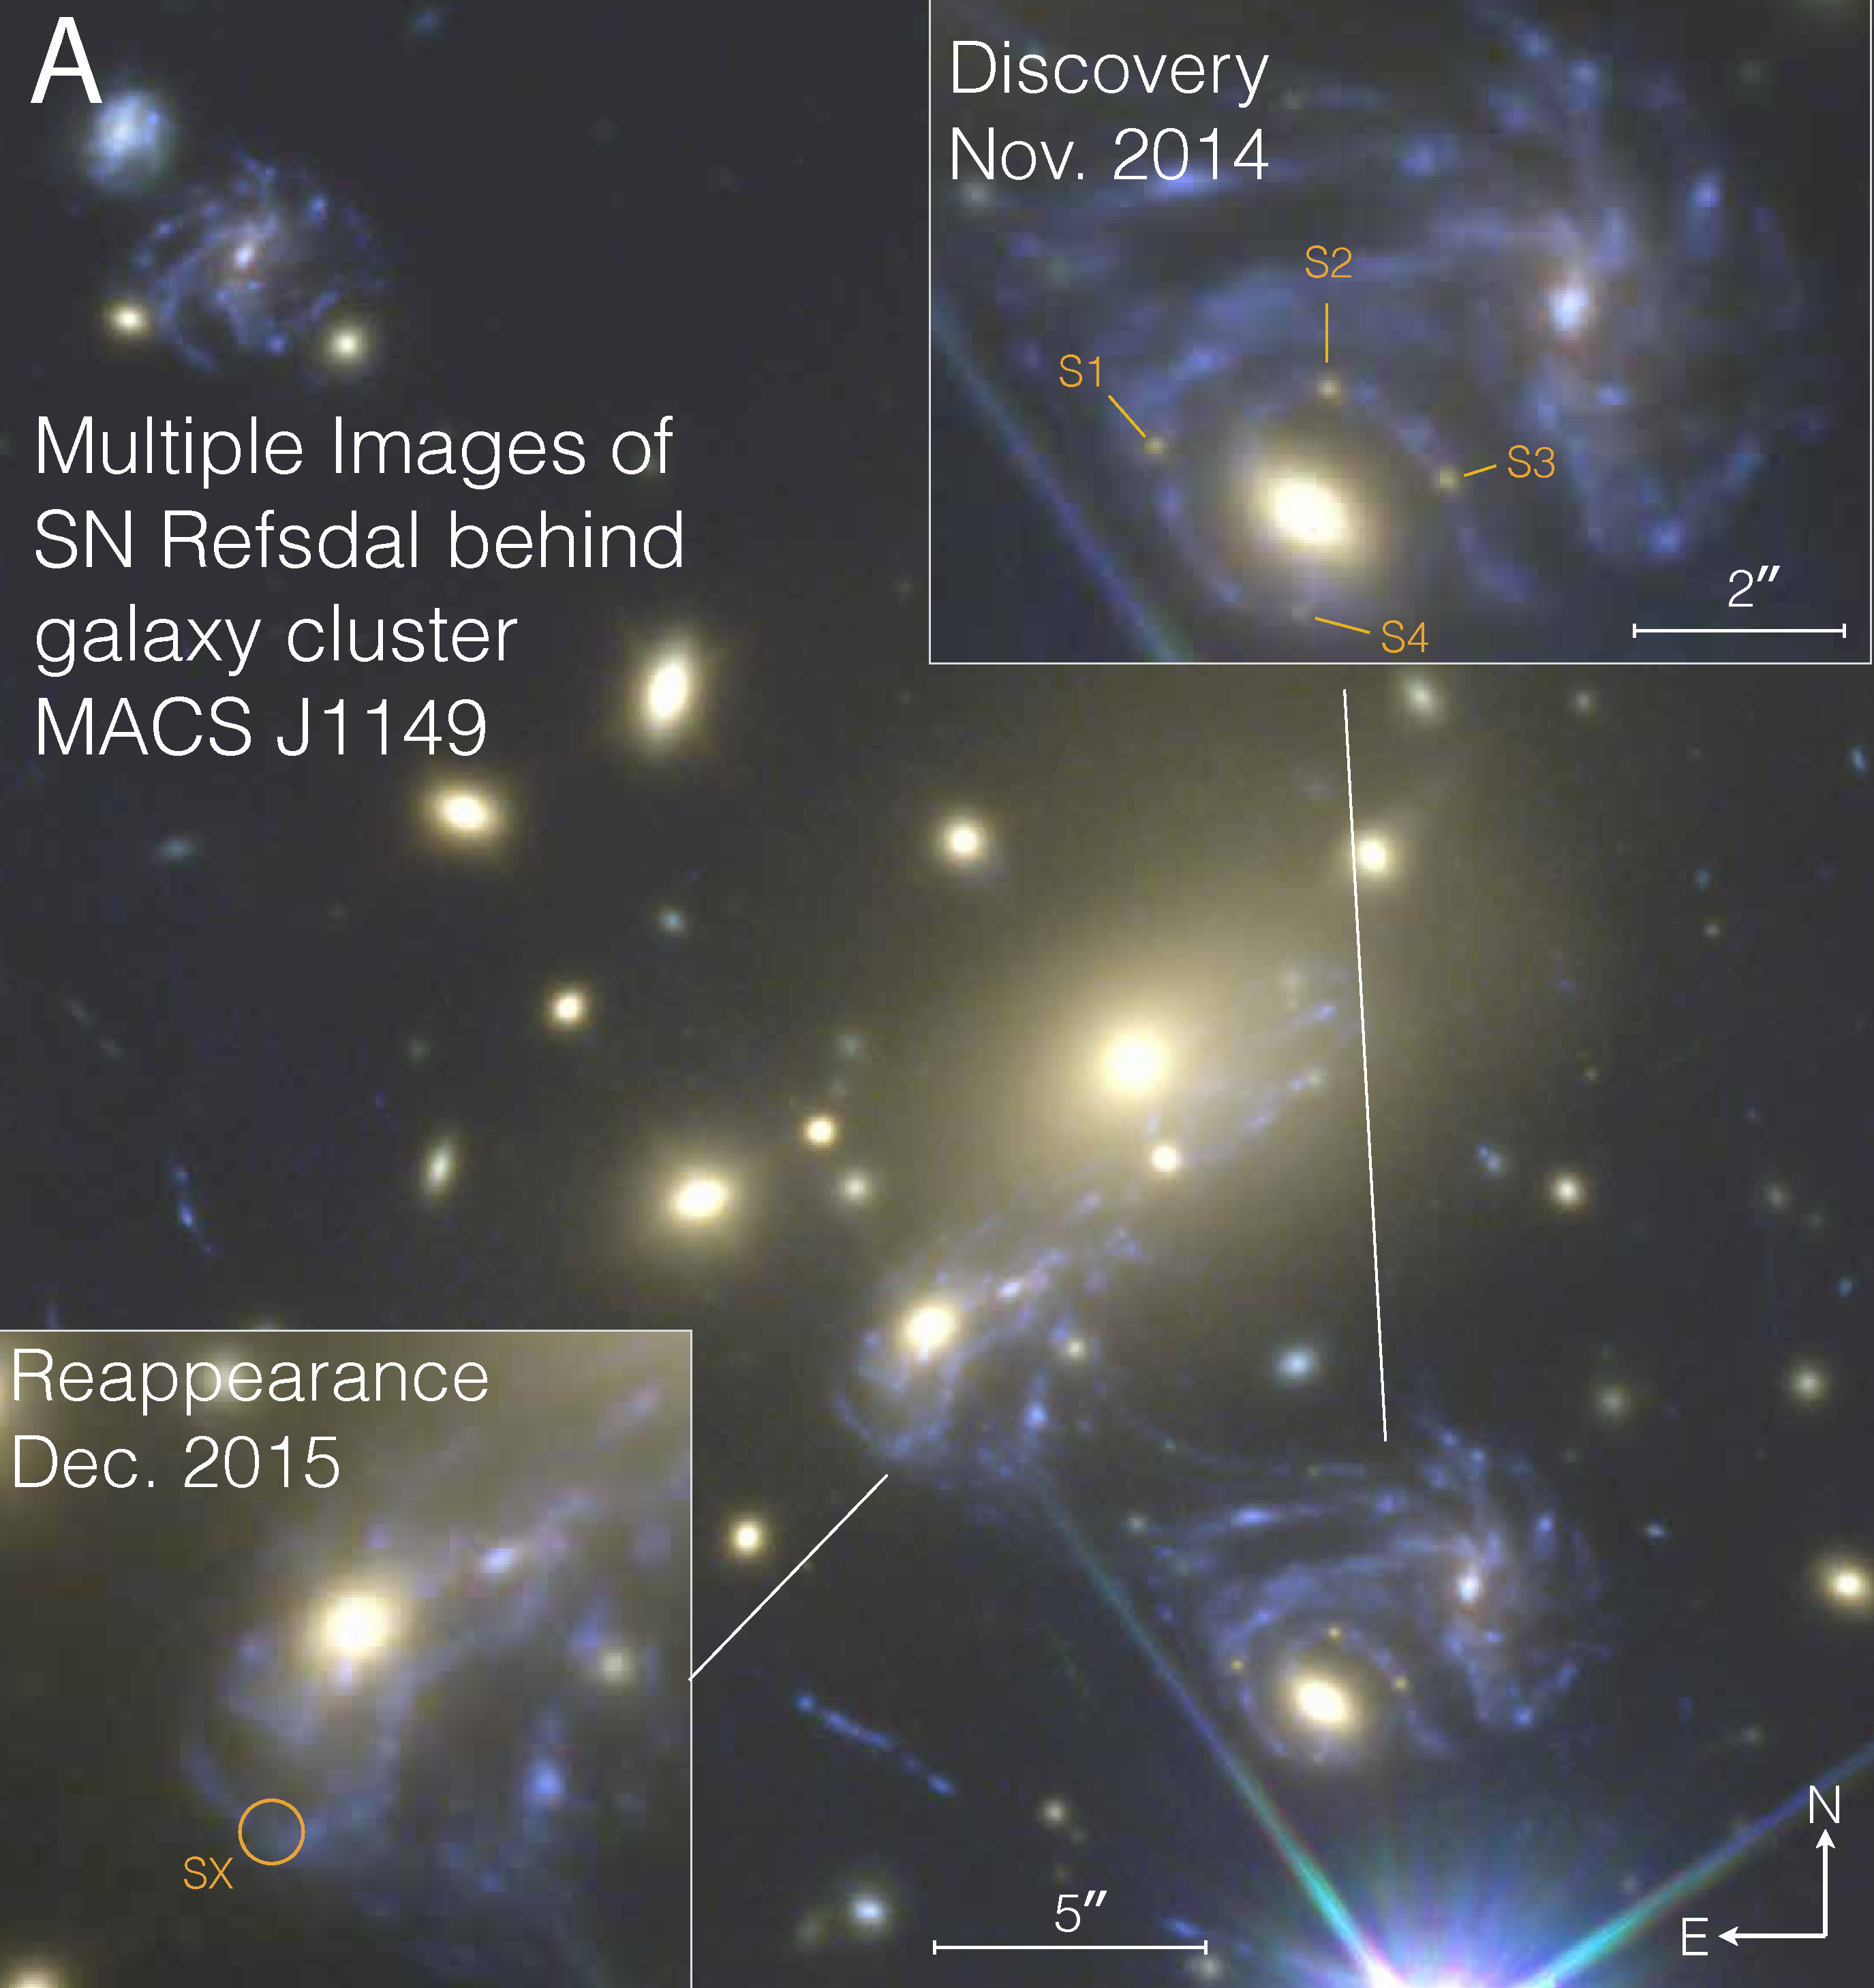
\includegraphics[height=.3\textwidth]{FIG/refsdal_summary2}
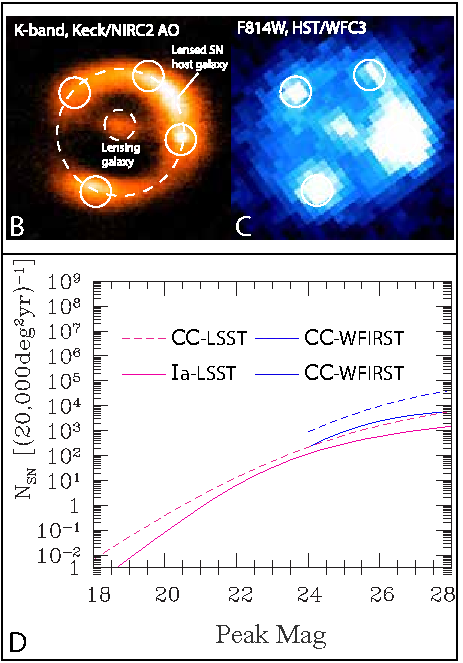
\includegraphics[height=.3\textwidth]{FIG/lensed3}
\caption{
(A) MACS J1149.6+2223 field, showing the positions of the three primary
images of the SN Refsdal host galaxy. SN
Refsdal appears as four point sources in an Einstein Cross
configuration in the southeast spiral arm of image 1.1. (B) HST/WFC3 observation
of iPTF16geu, revealing four point sources and (C) NIR Keck observation, with the 
Einstein ring of the host galaxy clearly visible, adapted from \citet{Goobar:2016}. (D)
Expected numbers of Type Ia and Core Collapse SNe for LSST $(i_{peak,lim})$ and 
WFIRST $(H_{peak,lim})$, adapted from \citet{Oguri:2010a}.}
\end{wrapfigure}

\noindent\underline{\textit{Intellectual Merit}} :
As the PI on an ongoing HST Archival Research Grant, \textbf{I am
developing the first open-source software package} in Python
(\textit{Supernova Time Delays} [SNTD]) that will enable a user to
precisely measure lens properties and time delays for the hundreds of
multiply imaged SNe expected in the LSST/WFIRST era (Figure 1D). I
will use SNTD to make more precise time delay measurements for the two
currently documented multiply imaged SNe. Properties of dark energy
and dark matter are still poorly understood and inadequately
constrained, but accurate measurement of the lensing magnification and
time delays for SN Refsdal can be used to test models for the dark
matter distribution in the lensing
object \citep{Rodney:2015a,Rodney:2016} or as a probe to test
cosmological models \citep{Suyu:2014}. As SN iPTF16geu is Type Ia,
providing more accurate time delay and luminosity distance
measurements will accomplish two critical goals. First, directly
measuring the source magnification will provide an important milestone
in breaking degeneracies in the lens
model \citep{Kolatt:1998,Oguri:2003b}. Second, precise determinations
of the time delays for a multiply imaged Type Ia SN will provide a
measurement of $H_0$ that is completely independent of the local
distance ladder, and the methodology and software I develop will
be \textbf{essential to future SN surveys} for tightening those
constraints.

Observations either by way of gravitational lensing, or by the next
generation telescope JWST, will provide a sample of extremely high
redshift SNe (Figure 2). Of interest in the early universe are
pair-instability (PI) and Population III (Pop III) SNe,
as \textbf{understanding these first stars is crucial to a wide range
of cosmology including the formation of primeval galaxies, initial
stages of cosmological reionization, and the origin of Supermassive
black holes} \citep{Whalen:2013}. Therefore, I will collect a sample
of high-z and gravitationally lensed SNe, and begin discerning
the properties of these poorly understood objects via powerful
lensing. With the SNe identified as weakly lensed, I will produce
careful magnification measurements and make small corrections
to the Hubble diagram. In addition to searching for PI and Pop III SNe
and studying their physical properties, I will include theoretical
light curve templates for both objects in SNTD, so that future
observations can be identified and both lens properties and progenitor
physics studied.

\begin{wrapfigure}{r}{.5\textwidth}
\centering
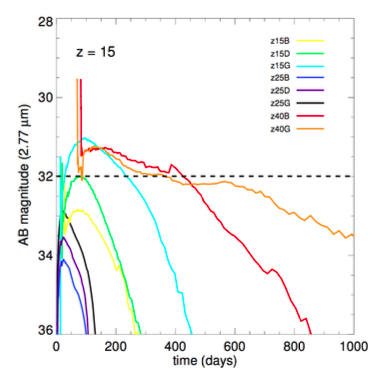
\includegraphics[height=.35\textwidth]{FIG/JWST_high_z}
\caption{
JWST will measure light curves for some of the earliest SN explosions
in the universe. Colored curves depict theoretical explosions from Pop
III SNe, and a dashed horizontal line shows the nominal detection
limit for JWST. These simulated light curves show that these first
stars are detectable by JWST, which makes their inclusion in SNTD
essential to future work (Figure adopted from \citet{Whalen:2013}).}
\end{wrapfigure}

\noindent\underline{\textit{Research Summary}}:
First, I will complete the python software package SNTD, and write a
publication presenting its capabilities and validation. Next I will
perform the reanalysis of SN Refsdal and SN iPTF16geu using SNTD,
writing a second publication presenting the more precise time delay
measurements, detailing the methodology required for these analyses,
and obtaining a constraint on $H_0$ from iPTF16geu. Finally, I will
add theoretical light curves for PISN and POP III SNe to the SNTD
package, and obtain a gravitationally lensed SN sample to study the
physics of these first stars. With the weaker lensed objects, I will
perform Hubble diagram magnification adjustments. From this last
component of my research, I will complete two further publications:
one describing magnification corrections for Hubble diagram SNe and
their affect on $H_0$, and the other detailing the search for, and
ideally discovery of, PISNe and POP III SNe and their physical
properties. These four publications will be a clear measure of the
success of this work, and the software and methodologies developed
during the course of my research will be vital for future work
using the next generation of space telescopes.

\noindent\underline{\textit{Broader Impacts Summary}}:
The SNTD software package will be a crucial tool in years to come, as
the next generation of telescopes drastically increases our catalogue
of multiply imaged SNe. Improving our understanding of the first stars
will be essential to various branches of cosmology such as the origin
of supermassive black holes, and I will pave the way for future PISN
and POP III SN observations by including their theoretical templates
in SNTD, and attempt to make \textbf{the first POP III SN observation}
by forming a sample of strongly lensed SNe. Finally, by documenting
SNTD and my improved measurement of the Refsdal and iPTF16geu time
delays, I will provide a measurement of $H_0$ and a standardized
methodology that will be used for future SN observations to tighten
constraints on $H_0$ and dark energy properties.

%\noindent\fontsize{10}{12}\selectfont
%some words
